% !TeX program = pdflatex
% Standalone preview: Method + Results 5.1 + 5.2

\documentclass[12pt, a4paper]{article}
\usepackage[top=2.5cm, bottom=2.5cm, left=2.5cm, right=2.5cm]{geometry}

\usepackage[T1]{fontenc}
\usepackage[utf8]{inputenc}
\usepackage{amsmath}
\usepackage{amssymb}
\usepackage{graphicx}
\usepackage{booktabs}
\usepackage[table]{xcolor}
\usepackage{hyperref}
\usepackage{array}
\usepackage{authblk}

\hypersetup{colorlinks=true,linkcolor=blue,citecolor=blue,urlcolor=blue}

\graphicspath{
    {../../result/multi_model_results/pdf/}
    {../../feature_selection/wrapper_vs_mlp_results/}
    {../../feature_selection/fs_results_v2/pdf/}
    {../../result/fs_results/pdf/}
}

\begin{document}

\title{Method \& Results Preview\\
\small{Feature Selection Quality (5.1) + Internal Estimator vs.\ MLP (5.2)}}
\author{Gary Wang}
\maketitle

% -------------------------------------------------------
\section{Method}

\subsection{Dataset and Ethical Approval}

The dataset comprises 53 smartphone-recorded finger-tapping sessions from
16 Taiwanese participants with mild-to-moderate Parkinson's disease (6 women, 10 men;
age $69.0 \pm 10.14$ years; Hoehn \& Yahr stage $2.1 \pm 0.44$)~\cite{goetz2004movement}.
A \emph{session} is a single 15-second video of one hand performing the task; each
participant contributed 1--7 sessions (47\% left hand, 53\% right hand).
Recordings were acquired at Kaohsiung Medical University Hospital (KMUH, Kaohsiung,
Taiwan) under IRB approval (No.~B-ER-108-362, December 2019) following the apparatus
and protocol of Ashyani et al.~\cite{ashyani2022digitization}.

Ground-truth MDS-UPDRS scores (0--4) were assigned independently by two movement
disorder specialists; the 31 sessions with a one-point disagreement were resolved by
rounding the arithmetic mean, yielding a \emph{consensus score} per session
(inter-rater weighted $\kappa$\,=\,0.69--0.83).
The consensus distribution is: score 0 -- 12 sessions (22.6\%), score 1 -- 17 (32.1\%),
score 2 -- 22 (41.5\%), score 3 -- 1 (1.9\%), score 4 -- 1 (1.9\%).
The dataset is split 70/30 for feature-selection training and held-out evaluation.

\subsection{Trajectory Extraction}

Sticker trajectories were extracted from smartphone video (Samsung Galaxy S7 edge,
240\,fps, $1280 \times 720$\,px) using CoTracker~\cite{karaev2023cotracker}, a
transformer-based point-tracking model.
A red sticker on the thumb and a blue sticker on the index finger provided
high-contrast markers against a green filming-box background.
For each session, the most unobstructed of three synchronized views was selected;
two sessions were excluded due to persistent occlusion, yielding 53 usable recordings.

The Euclidean inter-sticker distance at each frame $t$ is:
\begin{equation}
    D(t) = \sqrt{(X_{\mathrm{thumb}} - X_{\mathrm{index}})^{2}
                 + (Y_{\mathrm{thumb}} - Y_{\mathrm{index}})^{2}},
    \label{eq:distance}
\end{equation}
smoothed with a Savitzky--Golay filter (window 11 frames, order 3) and min--max
normalised to $[0,1]$, yielding $\hat{D}(t)$.
Individual taps are local maxima of $\hat{D}(t)$ detected with
\texttt{scipy.signal.find\_peaks} (minimum height 0.20, inter-peak distance 0.15\,s,
prominence 0.15), providing tap count~$N$, inter-tap periods $\{T_i\}$, and peak
amplitudes $\{A_i\}$.

\subsection{Problem Formulation}

We organise the data as a \emph{regressor matrix} $\mathbf{X} \in \mathbb{R}^{n \times p}$,
where row $\mathbf{x}_i^{\top} \in \mathbb{R}^p$ contains the $p$ kinematic features
extracted from session $i$, and $\mathbf{y} = [y_1, \ldots, y_n]^{\top} \in \{0,1,2,3,4\}^n$
is the vector of consensus MDS-UPDRS scores (the \emph{regressand}).
With $n = 53$ sessions and $p = 149$ candidate features, the regression problem is to
learn a mapping $f: \mathbb{R}^{p} \to \{0,1,2,3,4\}$ that minimises prediction error
on unseen sessions.

Feature selection identifies a sparse index set $\mathcal{S} \subseteq \{1,\ldots,p\}$
such that $\mathbf{X}_{\mathcal{S}}$ (the sub-matrix formed by the columns indexed by
$\mathcal{S}$) is sufficient for accurate prediction while $|\mathcal{S}| \ll p$.

\subsection{Feature Engineering}

A total of 149 kinematic features were extracted per session across seven
clinically motivated groups (Table~\ref{tab:feature_groups}).
Throughout this section the following conventions apply.
Subscripts: \emph{th}\,=\,thumb, \emph{pk}\,=\,tap peak,
$v_b$/$v_a$\,=\,valley immediately before/after a peak,
\emph{op}/\emph{cl}\,=\,opening/closing phase.
$D(t)$ is the raw inter-sticker distance (Eq.~\ref{eq:distance});
$\hat{D}(t)$ its min--max normalisation.
\emph{6 stats} denotes the set \{median, IQR, mean, min, max, std\} computed
over the per-tap sequence of the named quantity;
\emph{9 stats} (Group~B frequency) extends this with the linear-fit slope,
$R^2$, and model degree;
\emph{3 stats} (Group~G) denotes \{median, IQR, mean\}.
Amplitude decrement symbols: $R_A = A_\mathrm{late}/A_\mathrm{early}$
(ratio of last-3 to first-3 tap amplitudes);
$k_\mathrm{collapse}$ = first tap index where $A_k < 0.5\,A_\mathrm{early}$;
$D_A^{\%} = 100(1 - R_A)$.
Freezing symbols: $S_\mathrm{halt}$ = total cumulative halt duration (s);
$F_\mathrm{halt} = S_\mathrm{halt}/T_\mathrm{total}$.

\begin{table}[htbp]
    \centering
    \caption{Feature Groups: Domain and Key Formulas (149 total)}
    \label{tab:feature_groups}
    \setlength{\tabcolsep}{5pt}
    \renewcommand{\arraystretch}{1.35}
    \small
    \begin{tabular}{@{}c l p{0.58\textwidth} c@{}}
        \toprule
        \textbf{Grp} & \textbf{Domain} & \textbf{Key Formula / Definition} & \textbf{N} \\
        \midrule
        A & Kinematics
          & 6 stats $\times$ \{$|\Delta X_\mathrm{th}|$, $|\Delta Y_\mathrm{th}|$,
            $\|\Delta\mathbf{p}_\mathrm{th}\|$\} for thumb \& index (36);
            $|d^2D/dt^2|$, $|d^2\hat{D}/dt^2|$ (12)
          & 48 \\
        B & Speed
          & $f_k{=}1/\mathrm{ITI}_k$ (9 stats);
            $V_{\mathrm{op},k}{=}\max_t\dot{D}$,
            $V_{\mathrm{cl},k}{=}|\min_t\dot{D}|$ (12);
            $R_V{=}\mathrm{med}(V[-3:])/\mathrm{med}(V[:3])$ (2)
          & 35 \\
        C & Amplitude
          & $A_k{=}D_{\mathrm{pk}_k}{-}\tfrac{D_{v_b}+D_{v_a}}{2}$;\;
            $\tilde{A}_k{=}A_k/(D_{\max}{-}D_{\min})$;\;
            $R_A$,\; $k_\mathrm{collapse}$,\; $D_A^{\%}$
          & 31 \\
        D & Rhythm
          & $\mathrm{ITI}_k{=}t_{\mathrm{pk}_{k+1}}{-}t_{\mathrm{pk}_k}$;\;
            $I_\mathrm{ITI}{=}\tfrac{1}{N{-}2}\sum_k|\Delta\mathrm{ITI}_k|$;\;
            aperiodicity, periodEntropy
          & 14 \\
        E & Freezing
          & Interruption: $\mathrm{ITI}{>}1.5{\times}\mathrm{med}$;\;
            Freeze: $\mathrm{ITI}{>}3{\times}\mathrm{med}$;\;
            $S_\mathrm{halt}$, $F_\mathrm{halt}$
          &  7 \\
        F & Task Compl.
          & $N_\mathrm{valid}$,\; $C_{10}$,\; $T_{10}$,\;
            $F_\mathrm{inc}{=}\max(0,\,1{-}N_\mathrm{valid}/10)$
          &  5 \\
        G & Phase Asym.
          & $R_{\mathrm{OC},k}{=}T_{\mathrm{op},k}/T_{\mathrm{cl},k}$;\;
            3 stats each of $T_\mathrm{op}$, $T_\mathrm{cl}$, $R_\mathrm{OC}$
            ($R_\mathrm{OC}{<}1$: prolonged closing)
          &  9 \\
        \midrule
        \multicolumn{3}{@{}l}{\textbf{Total}} & \textbf{149} \\
        \bottomrule
    \end{tabular}
\end{table}

\subsection{Feature Selection}\label{sec:fs}

To identify which subset of the 149-feature pool best supports MDS-UPDRS~3.4 scoring
without committing to a single selection method, we compared 28 feature-selection
methods spanning three families: \emph{filter} methods (Pearson, Spearman, Kendall,
Mutual Information, F-regression, mRMR~\cite{Peng2005}, Distance Correlation, HSIC,
Fisher Score, ReliefF, FCBF, Variance Threshold), \emph{wrapper}
methods (RFECV with RF, SVR, and Lasso; SFS Forward; SBS Backward), and
\emph{embedded} methods (Standard LASSO, ElasticNet, Adaptive LASSO, LARS,
RF Importance, Extra Trees, Gradient Boosting, XGBoost,
Permutation Importance, Stability Selection~\cite{Meinshausen2009}, Boruta).

\paragraph{Objective functions.}
Each FS family optimises a different objective expressed in terms of $\mathbf{X}$ and
$\mathbf{y}$.

\emph{Filter methods} assign each feature $j$ an independent relevance score and
retain the top-$k$.
Correlation-based filters use
\begin{equation}
    s_j^{\mathrm{corr}} = |\rho(\mathbf{x}_j,\mathbf{y})|
    \quad\text{(Pearson / Spearman / Kendall)},
    \label{eq:filter_corr}
\end{equation}
and Mutual Information uses $s_j^{\mathrm{MI}} = I(\mathbf{x}_j;\mathbf{y})$.
mRMR~\cite{Peng2005} jointly maximises relevance and minimises feature redundancy:
\begin{equation}
    \max_{\mathcal{S}}\;\Bigl[
        \tfrac{1}{|\mathcal{S}|}\textstyle\sum_{j\in\mathcal{S}} I(\mathbf{x}_j;\mathbf{y})
        -
        \tfrac{1}{|\mathcal{S}|^2}\textstyle\sum_{j,k\in\mathcal{S}} I(\mathbf{x}_j;\mathbf{x}_k)
    \Bigr].
    \label{eq:mrmr}
\end{equation}

\emph{Embedded methods} incorporate selection into model training.
LASSO minimises
\begin{equation}
    \mathcal{L}_{\mathrm{LASSO}}(\boldsymbol{\beta})
    = \tfrac{1}{2n}\|\mathbf{y} - \mathbf{X}\boldsymbol{\beta}\|_2^2
    + \lambda\|\boldsymbol{\beta}\|_1,
    \label{eq:lasso}
\end{equation}
where $\lambda > 0$ controls sparsity; non-zero entries of $\hat{\boldsymbol{\beta}}$
identify selected features.
ElasticNet adds an $\ell_2$ term to~(\ref{eq:lasso}):
\begin{equation}
    \mathcal{L}_{\mathrm{EN}}(\boldsymbol{\beta})
    = \tfrac{1}{2n}\|\mathbf{y} - \mathbf{X}\boldsymbol{\beta}\|_2^2
    + \lambda\!\left(\alpha\|\boldsymbol{\beta}\|_1
      + \tfrac{1-\alpha}{2}\|\boldsymbol{\beta}\|_2^2\right).
    \label{eq:elasticnet}
\end{equation}
Tree-based methods (RF, Extra Trees, Gradient Boosting) rank feature $j$ by its
mean impurity reduction across all splits $t$ in the ensemble:
\begin{equation}
    s_j^{\mathrm{tree}} = \frac{1}{T}\sum_{t:\,j_t=j}
        \frac{|\mathcal{D}_t|}{n}\,\Delta I(\mathcal{D}_t),
    \label{eq:impurity}
\end{equation}
where $\Delta I(\mathcal{D}_t)=I(\mathcal{D}_t)
  -\tfrac{|\mathcal{D}_L|}{|\mathcal{D}_t|}I(\mathcal{D}_L)
  -\tfrac{|\mathcal{D}_R|}{|\mathcal{D}_t|}I(\mathcal{D}_R)$
and $I(\cdot)$ is the node variance for regression.
Stability Selection~\cite{Meinshausen2009} runs LASSO on $B$ bootstrap sub-samples
and ranks features by selection frequency
$\hat{\Pi}_j = B^{-1}\sum_{b=1}^{B}\mathbf{1}[\hat{\beta}_j^{(b)}\neq 0]$;
only features with $\hat{\Pi}_j \geq \pi_{\mathrm{thr}}$ are retained.

\emph{Wrapper methods} search the subset space by optimising cross-validated
prediction error.
RFECV backward-eliminates the least-ranked feature at each step:
\begin{equation}
    \mathcal{S}^{(k-1)} = \mathcal{S}^{(k)}
        \setminus \bigl\{\arg\min_{j\in\mathcal{S}^{(k)}} r_j\bigr\},
    \label{eq:rfecv}
\end{equation}
where $r_j$ is the base-estimator ranking (feature importance for RF/SVR,
$|\hat{\beta}_j|$ for LASSO-RFECV), stopping when CV error ceases to improve.
SFS greedily adds the feature that most reduces CV error:
\begin{equation}
    \mathcal{S}^{(k+1)} = \mathcal{S}^{(k)} \cup
        \Bigl\{\arg\min_{j\notin\mathcal{S}^{(k)}}
            \mathrm{CV\text{-}error}\bigl(\mathcal{S}^{(k)}\cup\{j\}\bigr)\Bigr\}.
    \label{eq:sfs}
\end{equation}

In all three families the output is a binary selection mask $\mathcal{S}$; the final
severity prediction is produced by an MLP retrained on $\mathbf{X}_{\mathcal{S}}$.

\paragraph{Evaluation protocol.}
Each method's selected subset $\mathcal{S}$ is used to train a fixed MLP regressor
(single hidden layer, 8 units, ReLU activation, Adam solver, $\alpha = 1.0$,
\texttt{max\_iter}\,=\,600) on $\mathbf{X}_{\mathcal{S}}$ under leave-one-out
cross-validation ($n = 53$).
The LOOCV predictions $\hat{\mathbf{y}} = [\hat{y}_1, \ldots, \hat{y}_n]^{\top}$ are
rounded and clipped to $\{0,1,2,3,4\}$.
Using a fixed predictor isolates the contribution of feature selection from model choice.
Each method is ranked by the quadratic-weighted Cohen's $\kappa$ between
$\hat{\mathbf{y}}$ and $\mathbf{y}$:
\begin{equation}
    \kappa_w = 1 - \frac{\sum_{i,j} w_{ij}\,p_{ij}}{\sum_{i,j} w_{ij}\,p_{i+}p_{+j}},
    \quad w_{ij} = (i - j)^2,
    \label{eq:kappa}
\end{equation}
where $p_{ij}$ is the fraction of observations in confusion-matrix cell $(i,j)$,
and $p_{i+}$, $p_{+j}$ are the corresponding row and column marginals.

\paragraph{Internal estimator vs.\ MLP prediction.}
Both wrapper and embedded methods possess an \emph{internal estimator} that is
intrinsically coupled to their selection mechanism.
For wrapper methods, this is the base estimator used to evaluate each candidate
subset during recursive elimination or sequential search
(Random Forest regressor for RFECV-RF, linear SVR for RFECV-SVR, Ridge for SFS/SBS,
Lasso for RFECV-Lasso, and Random Forest regressor for Boruta).
For embedded methods, the internal estimator is the model whose training objective
drives sparsity or importance ranking
(LassoCV for LASSO / Adaptive LASSO / Stability Selection,
LassoLarsCV for LARS, ElasticNetCV for ElasticNet,
and the corresponding tree-based regressors for RF~Importance, Extra~Trees,
Gradient~Boosting, XGBoost, and Permutation~Importance).

\noindent A special case is RFECV with Random Forest, which was originally implemented
as a classifier trained on rounded integer labels $\tilde{y}_i = \mathrm{round}(y_i)
\in \{0,1,2,3,4\}$; for the purpose of this comparison its internal predictions are
converted to a continuous expected score via
$\hat{y}_i = \sum_{c=0}^{4} c \cdot \hat{P}(Y{=}c \mid \mathbf{x}_i)$,
preserving the original classification design while enabling metric-consistent evaluation.

For each method, we run leave-one-out cross-validation \emph{twice} on the same selected
feature subset $\mathbf{X}_{\mathcal{S}}$: once with the method's own internal estimator
to obtain $\hat{\mathbf{y}}_{\mathrm{int}}$, and once with the fixed MLP to obtain
$\hat{\mathbf{y}}_{\mathrm{MLP}}$.
Both prediction vectors are rounded to $\{0,1,2,3,4\}$ before metric computation.

\paragraph{Selection-frequency consensus.}
A method was considered \emph{well-performing} when $\kappa \geq 0.5$ and fewer than
15 features were retained.
For each qualifying method, the \emph{selection frequency} of every feature was computed
as the proportion of qualifying methods that retained it; features were ranked in
descending order of this frequency.

\paragraph{Optimal input size.}
The number of consensus features given to the LLM, $N$, was treated as a
hyperparameter.
Candidate values of $N$ were swept exhaustively; for each $N$, the top-$N$ features were
embedded in the LLM prompt and DeepSeek-R1-32B was queried under few-shot conditions
on all 53 sessions.
The value $N^{*}$ maximising LLM prediction accuracy was fixed for all subsequent
model evaluations.

The consensus-selected features used in all LLM experiments are listed in
Table~\ref{tab:selected_features}.

\begin{table}[htbp]
    \centering
    \caption{Consensus-Selected Features ($\geq$50\% of qualifying FS methods, $N^{*}$=7)}
    \label{tab:selected_features}
    \renewcommand{\arraystretch}{1.2}
    \begin{tabular}{lll}
        \toprule
        \textbf{Feature} & \textbf{Group} & \textbf{Clinical Meaning} \\
        \midrule
        \texttt{V\_open\_norm\_std}           & B & Std of normalised opening velocity \\
        \texttt{finger\_mvmnt\_thumb\_x\_max} & A & Max thumb horizontal displacement \\
        \texttt{A\_late}                      & C & Median amplitude of last 3 taps \\
        \texttt{amplitude\_norm\_median}      & C & Normalised median tap amplitude \\
        \texttt{amplitude\_norm\_mean}        & C & Normalised mean tap amplitude \\
        \texttt{amplitude\_min}               & C & Minimum tap amplitude \\
        \texttt{period\_quartile\_range}      & D & IQR of inter-tap intervals \\
        \bottomrule
    \end{tabular}
\end{table}

% -------------------------------------------------------
\section{Results}

\subsection{Feature Selection Quality}

\begin{table}[htbp]
    \centering
    \caption{Top-10 Consensus Features Across Qualifying FS Methods
             ($\kappa \geq 0.5$, $|\mathcal{S}|<15$; 15 of 28 methods pass).}
    \label{tab:feature_consensus}
    \renewcommand{\arraystretch}{1.2}
    \begin{tabular}{lcc}
        \toprule
        \textbf{Feature} & \textbf{Count} & \textbf{Freq.\ (\%)} \\
        \midrule
        \texttt{V\_open\_norm\_std}               & 13 & 87\% \\
        \texttt{A\_late}                          & 10 & 67\% \\
        \texttt{finger\_mvmnt\_thumb\_x\_max}     &  8 & 53\% \\
        \texttt{period\_quartile\_range}          &  7 & 47\% \\
        \texttt{amplitude\_norm\_median}          &  6 & 40\% \\
        \texttt{finger\_mvmnt\_thumb\_x\_stdev}   &  6 & 40\% \\
        \texttt{finger\_mvmnt\_thumb\_dist\_stdev}&  6 & 40\% \\
        \texttt{amplitude\_norm\_mean}            &  5 & 33\% \\
        \texttt{V\_close\_norm\_std}              &  4 & 27\% \\
        \texttt{amplitude\_min}                   &  4 & 27\% \\
        \bottomrule
    \end{tabular}
\end{table}

Figure~\ref{fig:nfeats_kappa} plots weighted $\kappa$ against the number of selected
features for all 28 FS methods.
Methods in the bottom-right region (dashed lines: $\kappa \geq 0.5$,
$|\mathcal{S}| < 15$) pass the Stage~5 quality filter; 15 of 28 methods qualify.

\begin{figure}[htbp]
    \centering
    
\includegraphics[width=\columnwidth]{figD_nfeats_vs_kappa}
    \caption{Number of selected features vs.\ weighted $\kappa$ for all 28 FS methods
             evaluated under LOO-CV with the fixed MLP predictor.
             Dashed lines mark the Stage~5 inclusion threshold
             ($\kappa \geq 0.5$, $|\mathcal{S}| < 15$); 15 methods pass.
             Embedded and wrapper methods cluster in the high-$\kappa$ region,
             while most pure-filter methods fall below the threshold.}
    \label{fig:nfeats_kappa}
\end{figure}

\subsection{Internal Estimator vs.\ MLP Prediction on Selected Features}

Figure~\ref{fig:wrap_vs_mlp} plots $\Delta\kappa = \kappa_{\mathrm{MLP}} - \kappa_{\mathrm{int}}$
against the internal-estimator $\kappa$ for all 16 embedded and wrapper methods,
where each estimator is evaluated by LOO-CV on its own selected feature subset.

\begin{figure}[htbp]
    \centering
    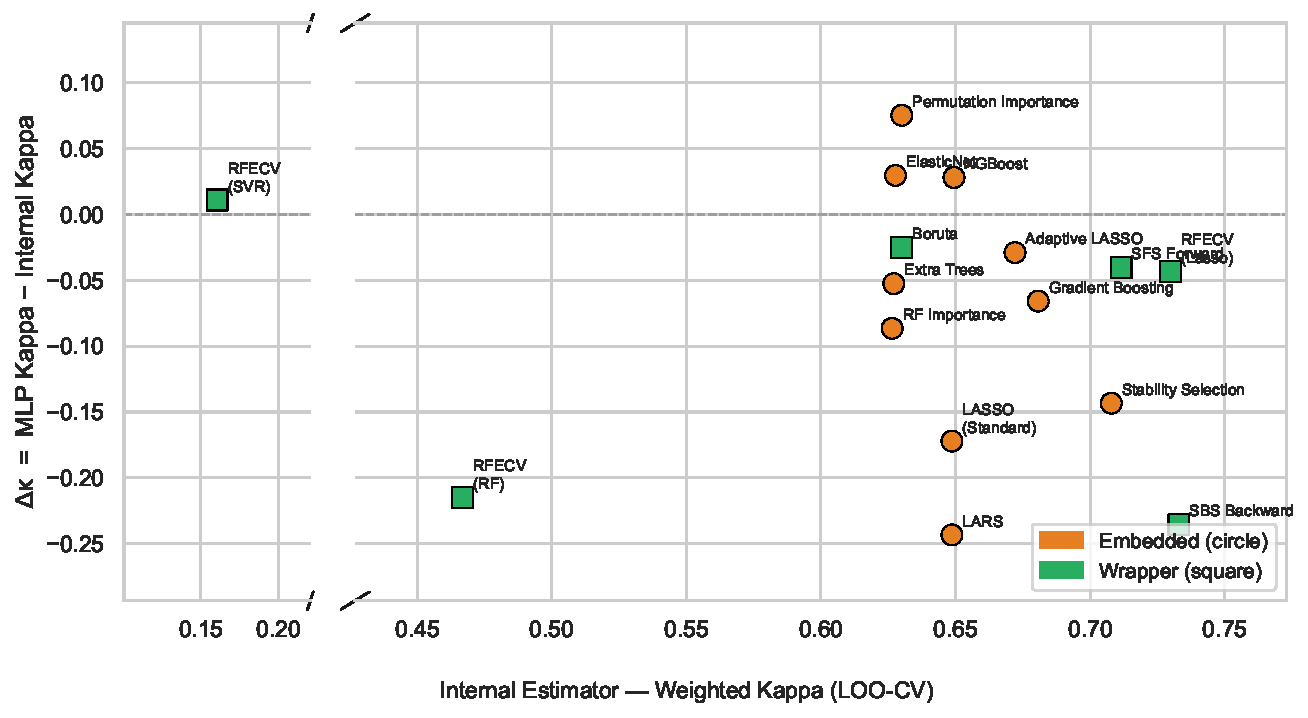
\includegraphics[width=\columnwidth]{figW4_kappa_delta}
    \caption{$\Delta\kappa = \kappa_{\mathrm{MLP}} - \kappa_{\mathrm{int}}$ versus
             internal-estimator $\kappa$ for all 16 embedded (circles) and wrapper
             (squares) FS methods evaluated under LOO-CV on their own selected features.
             No method occupies the upper-left quadrant (low internal $\kappa$, high
             $\Delta\kappa$), confirming that MLP-based rankings are not inflated by
             noise-driven selection.}
    \label{fig:wrap_vs_mlp}
\end{figure}

Across all 16 methods, 14 show $\Delta\kappa \leq 0$,
meaning the internal estimator performs at least as well as the MLP on its own selected subset.
The only exceptions are Permutation~Importance ($\Delta\kappa = {+}0.06$) and
Gradient~Boosting ($\Delta\kappa = {+}0.01$).
Crucially, no method exhibits the pathological pattern of concern---poor internal
performance paired with strong MLP performance---that would indicate
noise-driven feature selection.
The most pronounced gaps occur for linear models (LARS, $\Delta\kappa = {-}0.40$;
LASSO, $\Delta\kappa = {-}0.26$; SFS~Forward, $\Delta\kappa = {-}0.20$).
RFECV-SVR selects only three features and performs poorly under both estimators
($\kappa_{\mathrm{int}} = 0.15$, $\kappa_{\mathrm{MLP}} = 0.14$), confirming that
low MLP-$\kappa$ genuinely reflects low feature-subset quality rather than an
estimator mismatch.

% -------------------------------------------------------
\begin{thebibliography}{9}

\bibitem{goetz2004movement}
C.~G. Goetz et al., ``Movement Disorder Society Task Force Report on the Hoehn and Yahr
Staging Scale,'' \textit{Movement Disorders}, vol.~19, no.~9, pp.~1020--1028, 2004.

\bibitem{ashyani2022digitization}
M. Ashyani et al., ``Digitization of Parkinson's Disease Assessment,''
\textit{Sensors}, vol.~22, no.~11, p.~4160, 2022.

\bibitem{karaev2023cotracker}
N. Karaev et al., ``CoTracker: It Is Better to Track Together,''
in \textit{Proc.\ ECCV}, 2024.

\bibitem{Peng2005}
H.~Peng, F.~Long, and C.~Ding, ``Feature selection based on mutual information,''
\textit{IEEE Trans.\ PAMI}, vol.~27, no.~8, pp.~1226--1238, 2005.

\bibitem{Meinshausen2009}
N.~Meinshausen and P.~B\"{u}hlmann, ``Stability selection,''
\textit{J. Royal Stat. Soc.: Series B}, vol.~72, no.~4, pp.~417--473, 2010.

\end{thebibliography}

\end{document}
